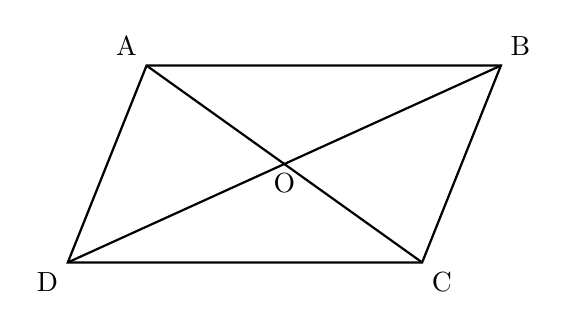
\begin{tikzpicture}[scale=1]

    % Define the coordinates for the vertices of the quadrilateral ABCD
    % D is the bottom-left vertex
    \coordinate (D) at (0, 0);
    % C is the bottom-right vertex
    \coordinate (C) at (4.5, 0);
    % B is the top-right vertex
    \coordinate (B) at (5.5, 2.5);
    % A is the top-left vertex
    \coordinate (A) at (1, 2.5);
    
    % Define the intersection point O (intersection of diagonals AC and BD)
    % Based on the parallelogram/rhombus properties
    \coordinate (O) at (2.75, 1.25);

    % Draw the four outer line segments of the shape (A-B, B-C, C-D, D-A)
    \draw[thick] (A) -- (B) -- (C) -- (D) -- cycle;

    % Draw the inner diagonal line segment from A to C
    \draw[thick] (A) -- (C);
    
    % Draw the inner diagonal line segment from B to D
    \draw[thick] (B) -- (D);

    % Add text labels for the vertices exactly as they appear in the image
    \node[above left] at (A) {A};
    \node[above right] at (B) {B};
    \node[below right] at (C) {C};
    \node[below left] at (D) {D};
    
    % Add the label for the intersection point O, placed slightly below the crossing
    \node[below] at (O) {O};

\end{tikzpicture}